\subsection{Debiased Contrastive Learning}\label{subsec:debiasing_cl}

\citet{chuang_debiased_2020} propose a debiased contrastive objective that corrects for sampling \acp{fn}, 
i.e., the selection of negative samples that have the same label as the anchor, in an unsupervised scenario.
They denote sampling bias the phenomenon where anchor $x$ and negative sample $x^-$ are similar to each other.
When randomly sampling negative samples from the data distribution $p(x)$ 
a negative sample can inherently belong to the same latent class as the anchor.
This phenomenon is illustrated in \autoref{fig:sampling_bias}a.
The effect of sampling bias on the model's performance is illustrated in \autoref{fig:sampling_bias}b.

\begin{figure}%
    \centering
    \subfloat[\centering Visualization of sampling bias similar to \citet{chuang_debiased_2020}. Sampling $x_i^-$ from $p$ can result in \ac{fn}.]
    {{\includegraphics[width=5cm]{images/sampling_bias.png} }}%
    \qquad
    \subfloat[\centering Negative influence of sampling bias on accuracy from \citet{chuang_debiased_2020}.]{{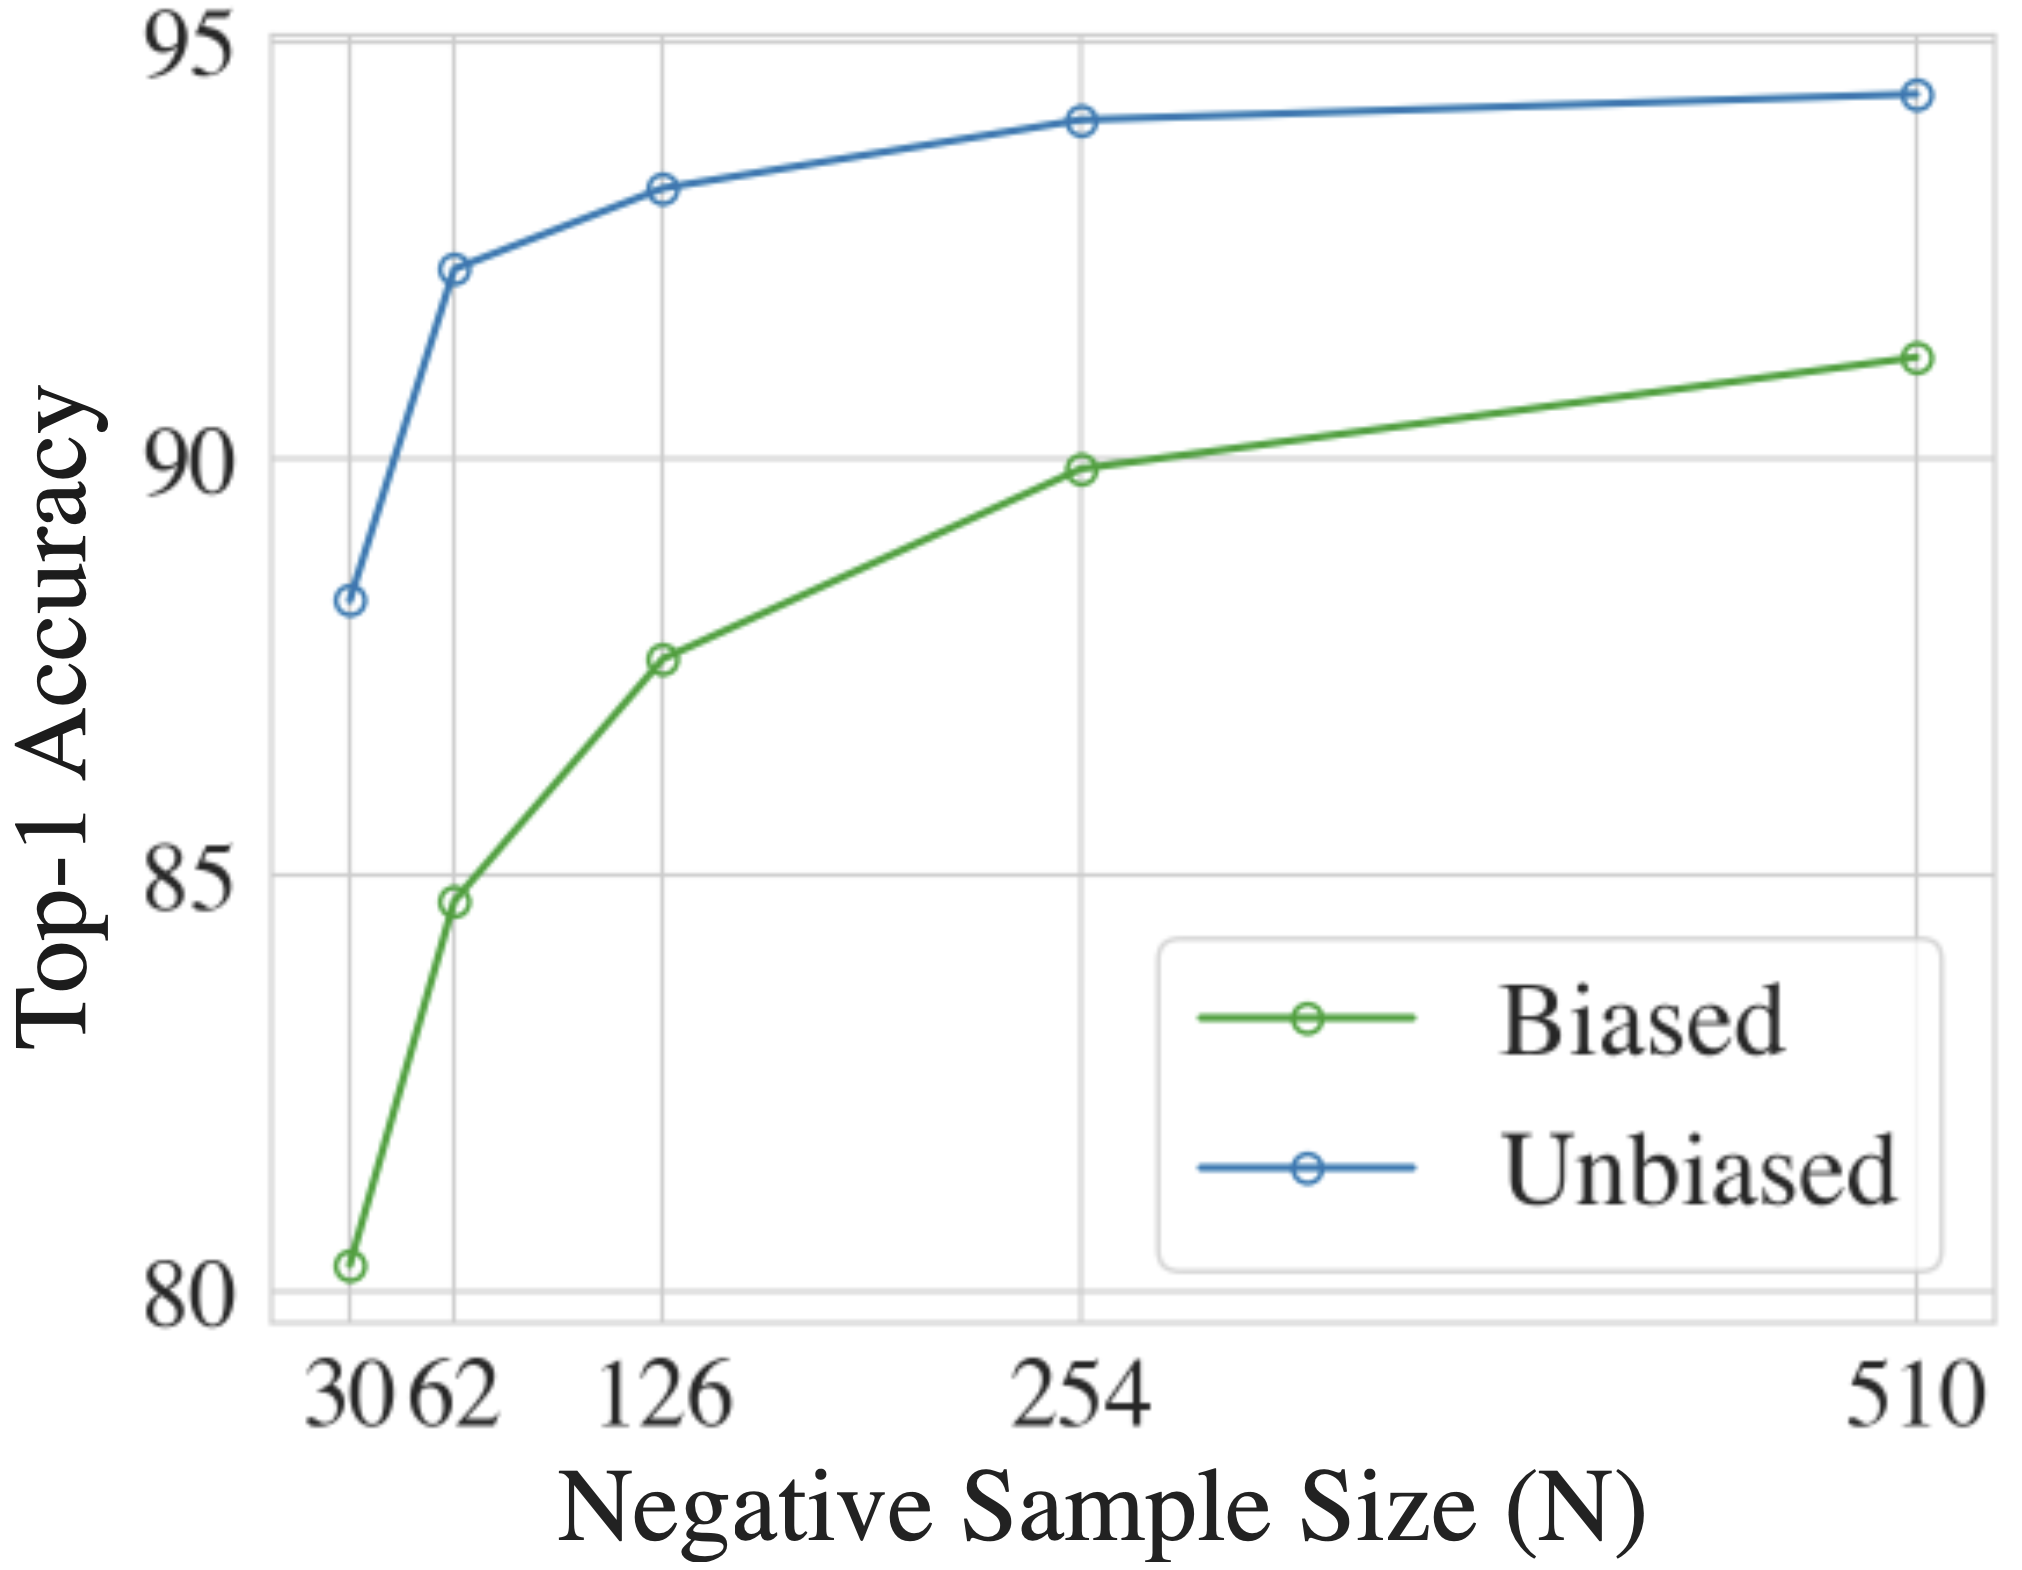
\includegraphics[width=5cm]{images/debiased_sampling_accuracy.png} }}%
    \caption{Visualization of sampling bias and its effect on the model's performance.}%
    \label{fig:sampling_bias}%
\end{figure}

\citeauthor{chuang_debiased_2020} assume a \ac{pu} learning scenario, 
where a positive sample and an unlabeled dataset $p(x)$ are available.
The positive distribution $p^+$ is mimicked by data augmentations.
The empirical estimation of the objective is given in 
\autoref{eq:debiasing_loss} from \citet{chuang_debiased_2020},
which is easier to compute than the original objective.
The negative samples $x^-$ are sampled from the data distribution $p(x)$.
However, the authors added a correction term for positive samples $v$.
The weighting factor $Q$ is used to balance the debiasing effect.

\begin{equation}
    \mathbb{E}_{x \sim p; x^+ \sim p^+}[{-\log{\frac{e^{f(x)^Tf(x^+)}}{e^{f(x)^Tf(x^+)}+ \frac{Q}{\tau^-}(\mathbb{E}_{x^- \sim p}[e^{f(x)^Tf(x^-)}]-\tau^+\mathbb{E}_{v \sim p^+}[e^{f(x)^Tf(v)}])}}}]
    \label{eq:debiasing_loss}
\end{equation}
